% SampleProject.tex -- main LaTeX file for sample LaTeX article
%
%\documentclass[12pt]{article}
\documentclass[11pt]{SelfArxOneColBMN}
% add the pgf and tikz support.  This automatically loads
% xcolor so no need to load color
\usepackage{pgf}
\usepackage{tikz}
\usetikzlibrary{matrix}
\usetikzlibrary{calc}
\usepackage{xstring}
\usepackage{pbox}
\usepackage{etoolbox}
\usepackage{marginfix}
\usepackage{xparse}
\setlength{\parskip}{0pt}% fix as marginfix inserts a 1pt ghost parskip
% standard graphics support
\usepackage{graphicx,xcolor}
\usepackage{wrapfig}
%
\definecolor{color1}{RGB}{0,0,90} % Color of the article title and sections
\definecolor{color2}{RGB}{0,20,20} % Color of the boxes behind the abstract and headings
%----------------------------------------------------------------------------------------
%	HYPERLINKS
%----------------------------------------------------------------------------------------
\usepackage[pdftex]{hyperref} % Required for hyperlinks
\hypersetup{hidelinks,
colorlinks,
breaklinks=true,%
urlcolor=color2,%
citecolor=color1,%
linkcolor=color1,%
bookmarksopen=false%
,pdftitle={SampleProject},%
pdfauthor={Peterson}}
%\usepackage[round,numbers]{natbib}
\usepackage[numbers]{natbib}
\usepackage{lmodern}
\usepackage{setspace}
\usepackage{xspace}
%
\usepackage{subfigure}
\newcommand{\goodgap}{
  \hspace{\subfigtopskip}
  \hspace{\subfigbottomskip}}
%
\usepackage{atbegshi}
%
\usepackage[hyper]{listings}
%
% use ams math packages
\usepackage{amsmath,amsthm,amssymb,amsfonts}
\usepackage{mathrsfs}
%
% use new improved Verbatim
\usepackage{fancyvrb}
%
\usepackage[titletoc,title]{appendix}
%
\usepackage{url}
%
% Create length for the baselineskip of text in footnotesize
\newdimen\footnotesizebaselineskip
\newcommand{\test}[1]{%
 \setbox0=\vbox{\footnotesize\strut Test \strut}
 \global\footnotesizebaselineskip=\ht0 \global\advance\footnotesizebaselineskip by \dp0
}
%
\usepackage{listings}

\DeclareGraphicsExtensions{.pdf, .jpg, .tif,.png}

% make sure we don't get orphaned words if at top of page
% or orphans if at bottom of page
\clubpenalty=9999
\widowpenalty=9999
\renewcommand{\textfraction}{0.15}
\renewcommand{\topfraction}{0.85}
\renewcommand{\bottomfraction}{0.85}
\renewcommand{\floatpagefraction}{0.66}
%
\DeclareMathOperator{\sech}{sech}

\newcommand{\mycite}[1]{%
(\citeauthor{#1} \citep{#1} \citeyear{#1})\xspace
}

\newcommand{\mycitetwo}[2]{%
(\citeauthor{#2} \citep[#1]{#2} \citeyear{#2})\xspace
}

\newcommand{\mycitethree}[3]{%
(\citeauthor{#3} \citep[#1][#2]{#3} \citeyear{#3})\xspace
}

\newcommand{\myincludegraphics}[3]{% file name, width, height
\includegraphics[width=#2,height=#3]{#1}
}

\newcommand{\myincludegraphicstwo}[2]{% file name, width, height
\includegraphics[scale=#1]{#2}
}

\newcommand{\mysimplegraphics}[1]{% file name, width, height
\includegraphics{#1}
}

\newcommand{\MB}[1]{
\boldsymbol{#1}
}

\newcommand{\myquotetwo}[1]{%
\small
%\singlespacing
\begin{quotation}
#1
\end{quotation}
\normalsize
%\onehalfspacing  
}

\newcommand{\jimquote}[1]{%
\small
%\singlespacing
\begin{quotation}
#1
\end{quotation}
\normalsize
%\onehalfspacing
}

\newcommand{\myquote}[1]{%
\small
%\singlespacing
\begin{quotation}
#1
\end{quotation}
\normalsize
%\onehalfspacing  
}

%A =
%
%[2 r_1 	     r_1]
%[-2r_1 + r_2  r_2 - r_1]
%
%has eigenvalues r_1 neq r_2.
% #1 = 2 r_1, #2 = r_1, #3 = -2r_1+r_2, #4 = r_2 - r_1
\newcommand{\myrealdiffA}[4]{
\left [
\begin{array}{rr}
#1  & #2\\
#3  & #4
\end{array}
\right ]
}

% args:
% 1, 2 ,3, 4, 5 = caption, label, width, height, file name
%\mysubfigure{}{}{}{}{}
\newcommand{\mysubfigure}[5]{%
\subfigure[#1]{\label{#2}\includegraphics[width=#3,height=#4]{#5}}
}

\newcommand{\mysubfiguretwo}[3]{%
\subfigure[#1]{\label{#2}\includegraphics{#3}}
}

\newcommand{\mysubfigurethree}[4]{%
\subfigure[#1]{\label{#2}\includegraphics[scale=#3]{#4}}
}

\newcommand{\myputimage}[5]{% file name, width, height
\centering
\includegraphics[width=#3,height=#4]{#5}
\caption{#1}
\label{#2}
}

\newcommand{\myputimagetwo}[4]{% caption, label, scale, file name
\centering
\includegraphics[scale=#3]{#4}
\caption{#1}
\label{#2}
}

\newcommand{\myrotateimage}[5]{% file name, width, height
\centering
\includegraphics[scale=#3,angle=#4]{#5}
\caption{#1}
\label{#2}
}

\newcommand{\myurl}[2]{%
\href{#1}{\bf #2}
}

\RecustomVerbatimEnvironment%
{Verbatim}{Verbatim}  
  {fillcolor=\color{black!20}}
  
  \DefineVerbatimEnvironment%
{MyVerbatim}{Verbatim}  
  {frame=single,
   framerule=2pt,
   fillcolor=\color{black!20},
   fontsize=\small}
   
\newcommand{\myfvset}[1]{%  
\fvset{frame=single,
       framerule=2pt,
       fontsize=\small,
       xleftmargin=#1in}}
       
\newcommand{\mylistverbatim}{%
\lstset{%
  fancyvrb, 
  basicstyle=\small,
  breaklines=true}
}  

\newcommand{\mylstinlinebf}[1]{%
{\bf #1}
}

\newcommand{\mylstinline}{%
\lstset{%
  basicstyle=\color{black!80}\bfseries\ttfamily,
  showstringspaces=false,
  showspaces=false,showtabs=false,
  breaklines=true}
\lstinline
}

\newcommand{\mylstinlinetwo}[1]{%
\lstset{%
  basicstyle=\color{black!80}\bfseries\ttfamily,
  showstringspaces=false,
  showspaces=false,showtabs=false,
  breaklines=true}
\lstinline!#1! 
}

%fontfamily=tt
%fontfamily=courier
%fontfamily=helvetica
%frame=topline,
%frame=single,
 %frame=lines,
 %framesep=10pt,
 %fontshape=it,
 %fontseries=b,
 %fontsize=\relsize{-1},
 %fillcolor=\color{black!20},
 %rulecolor=\color{yellow},
 %fillcolor=\color{red}
 %label=\fbox{\Large\emph{The code}}
\DefineVerbatimEnvironment%
{MyListVerbatim}{Verbatim}  
{
fillcolor=\color{black!10},
fontfamily=courier,
frame=single,
%formatcom=\color{white},
framesep=5mm,
labelposition=topline,
fontshape=it,
fontseries=b,
fontsize=\small,
label=\fbox{\large\emph{The code}\normalsize}
} 

%  caption={[#1] \large\bf{#1}}, 
%\centering \framebox[.6\textwidth][c]{\Large\bf{#1}}
\newcommand{\myfancyverbatim}[1]{%
\lstset{%
  fancyvrb=true, 
  %fvcmdparams= fillcolor 1,
  %morefvcmdparams = \textcolor 2,
  frame=shadowbox,framerule=2pt, 
  basicstyle=\small\bfseries,
  backgroundcolor=\color{black!08},
  showstringspaces=false,
  showspaces=false,showtabs=false,
  keywordstyle=\color{black}\bfseries,
  %numbers=left,numberstyle=\tiny,stepnumber=5,numbersep=5pt,
  stringstyle=\ttfamily,
  caption={[\quad #1] \mbox{}\\ \vspace{0.1in} \framebox{\large \bf{#1} \small} },  
  belowcaptionskip=20 pt,  
  label={},
  xleftmargin=17pt,
  framexleftmargin=17pt,
  framexrightmargin=5pt,
  framexbottommargin=4pt,
  nolol=false,
  breaklines=true}
}

\newcommand{\mylistcode}[3]{%
\lstset{%
  language=#1, 
  frame=shadowbox,framerule=2pt, 
  basicstyle=\small\bfseries,
  backgroundcolor=\color{black!16},
  showstringspaces=false,
  showspaces=false,showtabs=false,
  keywordstyle=\color{black!40}\bfseries,
  numbers=left,numberstyle=\tiny,stepnumber=5,numbersep=5pt,
  stringstyle=\ttfamily,
  caption={[\quad#2] \mbox{}\\ \vspace{0.1in} \framebox{\large \bf{#2} \small} },
  belowcaptionskip=20 pt,
  breaklines=true,
  xleftmargin=17pt,
  framexleftmargin=17pt,
  framexrightmargin=5pt,
  framexbottommargin=4pt,  
  label=#3,
  breaklines=true} 
}

  %caption={[#2] #3},
  %caption={[#2]{\mbox{}\\ \vspace{0.1in} \framebox{\large \bf{#3} \small}},
  %caption={[#2] \mbox{}\\ \bf{#3} },

% frame=single,
% caption={[Code Fragment] {\bf Code Fragment} },
% caption={[Code Fragment] \mbox{}\\ \vspace{0.1in} \framebox{\large \bf{Code Fragment} \small} },
\newcommand{\mylistcodequick}[1]{%
\lstset{%
  language=#1, 
  frame=shadowbox,framerule=2pt, 
  basicstyle=\small\bfseries,
  backgroundcolor=\color{black!16},
  showstringspaces=false,
  showspaces=false,showtabs=false,
  keywordstyle=\color{black!40}\bfseries,
  numbers=left,numberstyle=\tiny,stepnumber=5,numbersep=5pt,
  stringstyle=\ttfamily,
  caption={[\quad Code Fragment] \large \bf{Code Fragment} \small},   
  belowcaptionskip=20 pt,  
  label={},
  xleftmargin=17pt,
  framexleftmargin=17pt,
  framexrightmargin=5pt,
  framexbottommargin=4pt,
  breaklines=true} 
}

%  caption={[#2] \mbox{}\\ \vspace{0.1in} \framebox{\large \bf{#2} \small} },
\newcommand{\mylistcodequicktwo}[2]{%
\lstset{%
  language=#1, 
  frame=shadowbox,framerule=2pt, 
  basicstyle=\small\bfseries,
  extendedchars=true,
  backgroundcolor=\color{black!16},
  showstringspaces=false,
  showspaces=false,
  showtabs=false,
  keywordstyle=\color{black!40}\bfseries,
  numbers=left,numberstyle=\tiny,stepnumber=5,numbersep=5pt,
  stringstyle=\ttfamily,
  caption={[\quad#2] \large \bf{#2} \small},
  belowcaptionskip=20 pt,
  label={},
  xleftmargin=17pt,
  framexleftmargin=17pt,
  framexrightmargin=5pt,
  framexbottommargin=4pt,
  breaklines=true} 
}

%  caption={[#2] \mbox{}\\ \vspace{0.1in} \framebox{\large \bf{#2} \small} },
\newcommand{\mylistcodequickthree}[2]{%
\lstset{%
  language=#1, 
  frame=shadowbox,framerule=2pt, 
  basicstyle=\small\bfseries,
  extendedchars=true,
  backgroundcolor=\color{black!16},
  showstringspaces=false,
  showspaces=false,
  showtabs=false,
  keywordstyle=\color{black!40}\bfseries,
  numbers=left,numberstyle=\tiny,stepnumber=5,numbersep=5pt,
  stringstyle=\ttfamily,
  caption={[\quad#2] \large\bf{#2}\small},
  belowcaptionskip=20 pt,
  label={},
  xleftmargin=17pt,
  framexleftmargin=17pt,
  framexrightmargin=5pt,
  framexbottommargin=4pt,
  breaklines=true} 
}

%  frame=single,
\newcommand{\mylistset}[4]{%
\lstset{language=#1,
  basicstyle=\small,
  showstringspaces=false,
  showspaces=false,showtabs=false,
  keywordstyle=\color{black!40}\bfseries,
  numbers=left,numberstyle=\tiny,stepnumber=5,numbersep=5pt,
  stringstyle=\ttfamily,
  caption={[\quad#2]#3},
  label=#4}
}

\newcommand{\mylstinlineset}{%
\lstset{%
  basicstyle=\color{blue}\bfseries\ttfamily,
  showstringspaces=false,
  showspaces=false,showtabs=false,
  breaklines=true}
}

\newcommand{\myframedtext}[1]{%
\centering
\noindent
%\fbox{\parbox[c]{.9\textwidth}{\color{black!40} \small \singlespacing #1\onehalfspacing \normalsize \\}}
\fbox{\parbox[c]{.9\textwidth}{\color{black!40} \small  #1 \normalsize \\}}
}

\newcommand{\myemptybox}[2]{% from , to
\fbox{\begin{minipage}[t][#1in][c]{#2in}\hspace{#2in}\end{minipage}}
}

\newcommand{\myemptyboxtwo}[2]{% from , to
\centering\fbox{
\begin{minipage}{#1in}
\hfill\vspace{#2in}
\end{minipage}
}
}

\newcommand{\boldvector}[1]{
\boldsymbol{#1}
}

\newcommand{\dEdY}[2]{\frac{d E}{d Y_{#1}^{#2}}}
\newcommand{\dEdy}[2]{\frac{d E}{d y_{#1}^{#2}}}
\newcommand{\dEdT}[2]{\frac{\partial E}{\partial T_{{#1} \rightarrow {#2}}}}
\newcommand{\dEdo}[1]{\frac{\partial E}{\partial o^{#1}}}
\newcommand{\dEdg}[1]{\frac{\partial E}{\partial g^{#1}}}
\newcommand{\dYdY}[4]{\frac{\partial Y_{#1}^{#2}}{\partial Y_{#3}^{#4}}}
\newcommand{\dYdy}[4]{\frac{\partial Y_{#1}^{#2}}{\partial y_{#3}^{#4}}}
\newcommand{\dydY}[4]{\frac{\partial y_{#1}^{#2}}{\partial Y_{#3}^{#4}}}
\newcommand{\dydy}[4]{\frac{\partial y_{#1}^{#2}}{\partial y_{#3}^{#4}}}
\newcommand{\dydT}[4]{\frac{\partial y_{#1}^{#2}}{\partial T_{{#3} \rightarrow {#4}}}}
\newcommand{\dYdT}[4]{\frac{\partial Y_{#1}^{#2}}{\partial T_{{#3} \rightarrow {#4}}}}
\newcommand{\dTdT}[4]{\frac{\partial T_{{#1} \rightarrow {#2}}}{\partial T_{{#3} \rightarrow {#4}}}}
\newcommand{\ssum}[2]{\sum_{#1}^{#2}}

\newcommand{\ssty}[1]{\scriptscriptstyle #1}

\newcommand{\myparbox}[2]{%
\parbox{#1}{\color{black!20} #2}
}

\newcommand{\bs}[1]{
\boldsymbol{#1}
}

\newcommand{\parone}[2]{%
\frac{\partial #1 }{ \partial #2 }
}
\newcommand{\partwo}[2]{%
\frac{ \partial^2 {#1} }{ \partial {#2}^2 }
}

\newcommand{\twodvectorvarfun}[2]{
\left [
\begin{array}{r}
{{#1_{\ssty{1}}}(#2)} \\
{{#1_{\ssty{2}}}(#2)}
\end{array}
\right ]
}
\newcommand{\twodvectorvarprimed}[1]{
\left [
\begin{array}{r}
{{#1_{\ssty{1}}}'(t)} \\
{{#1_{\ssty{2}}}'(t)}
\end{array}
\right ]
}

\newcommand{\complex}[2]{#1 \: #2 \: \boldsymbol{i}}
\newcommand{\complexmag}[2]%
{
\sqrt{(#1)^2 \: + \: (#2)^2}
}
\newcommand{\threenorm}[3]%
{
\sqrt{(#1)^2 \: + \: (#2)^2 \: + \: (#3)^2}
}
\newcommand{\norm}[1]{\mid \mid #1 \mid \mid}

\newcommand{\myderiv}[2]{\frac{d #1}{d #2}}
\newcommand{\myderivb}[2]{\frac{d}{d #2} \left ( #1 \right )}
\newcommand{\myrate}[3]%
{#1^\prime(#2) &=& #3 \: #1(#2)
}
\newcommand{\myrateexter}[4]%
{#1^\prime(#2) &=& #3 \: #1(#2) \: + \: #4
}
\newcommand{\myrateic}[3]%
{#1( \: #2 \:) &=& #3 
}

\newcommand{\mytwodsystemeqn}[6]{
#1 \: x    #2 \: y &=& #3\\
#4 \: x    #5 \: y &=& #6\\
}

\newcommand{\mytwodsystem}[8]{
#3 \: #1 \: + \: #4 \: #2 &=& #5\\
#6 \: #1 \: + \: #7 \: #2 &=& #8\\
}  

\newcommand{\mytwodarray}[4]{
\left [
\begin{array}{rr}
#1 & #2\\
#3 & #4
\end{array}
\right ]
}

\newcommand{\mytwoid}{
\left [
\begin{array}{rr}
1 & 0\\
0 & 1
\end{array}
\right ]
}

\newcommand{\myxprime}[2]{
\left [
\begin{array}{r}
#1^\prime(t)\\
#2^\prime(t)
\end{array}
\right ]
}

\newcommand{\myxprimepacked}[2]{
\left [
\begin{array}{r}
#1^\prime\\
#2^\prime
\end{array}
\right ]
}

\newcommand{\myx}[2]{
\left [
\begin{array}{r}
#1(t)\\
#2(t)
\end{array}
\right ]
}

\newcommand{\myxonly}[2]{
\left [
\begin{array}{r}
#1\\
#2
\end{array}
\right ]
}

\newcommand{\myv}[2]{
\left [
\begin{array}{r}
#1\\
#2
\end{array}
\right ]
}

\newcommand{\myxinitial}[2]{
\left [
\begin{array}{r}
#1(0)\\
#2(0)
\end{array}
\right ]
}

\newcommand{\twodboldv}[1]{
\boldsymbol{#1}
}

\newcommand{\mytwodvector}[2]{
\left [
\begin{array}{r}
#1\\
#2
\end{array}
\right ]
}

\newcommand{\mythreedvector}[3]{
\left [
\begin{array}{r}
#1\\
#2\\
#3
\end{array}
\right ]
}

\newcommand{\mytwodsystemvector}[6]{
\left [
\begin{array}{rr}
#1 & #2\\
#4 & #5
\end{array}
\right ]
\:
\left [
\begin{array}{r}
x \\
y 
\end{array}
\right ]
&=&
\left [
\begin{array}{r}
#3\\
#6
\end{array}
\right ]
}

\newcommand{\mythreedarray}[9]{
\left [
\begin{array}{rrr}
#1 & #2 & #3\\
#4 & #5 & #6\\
#7 & #8 & #9
\end{array}
\right ]
}

\newcommand{\myodetwo}[6]{
#1 \: #6^{\prime \prime}(t) \: #2 \: #6^{\prime}(t) \: #3 \: #6(t) &=& 0\\
#6(0)                                           &=& #4\\
#6^{\prime}(0)                                  &=& #5
}

\newcommand{\myodetwoNoIC}[4]{
#1 \: #4^{\prime \prime}(t) \: #2 \: #4^{\prime}(t) \: #3 \: #4(t) &=& 0
}

\newcommand{\myodetwopacked}[5]{
\hspace{-0.3in}& & #1 u^{\prime \prime} #2 u^{\prime} #3 u \: = \: 0\\
\hspace{-0.3in}& & u(0) \: = \: #4, \: \: u^{\prime}(0)    \: = \:  #5
}

\newcommand{\myodetwoforced}[6]{
#1\: u^{\prime \prime}(t) \: #2 \: u^{\prime}(t) \: #3 \: u(t) &=& #6\\
u(0)                                           &=& #4\\
u^{\prime}(0)                                  &=& #5\\
}

\newcommand{\myodesystemtwo}[8]{
#1 \: x^\prime(t) \: #2 \: y^\prime(t) \: #3 \: x(t) \: #4 \: y(t) &=& 0\\
#5 \: x^\prime(t) \: #6 \: y^\prime(t) \: #7 \: x(t) \: #8 \: y(t) &=& 0\\
}

\newcommand{\myodesystemtwoic}[2]{
x(0)                                       &=& #1\\ 
y(0)                                       &=& #2
}

\newcommand{\mypredprey}[4]{
x^\prime(t) &=& #1 \: x(t) \: - \: #2 \: x(t) \: y(t)\\
y^\prime(t) &=& -#3 \: y(t) \: + \: #4 \: x(t) \: y(t)
}

\newcommand{\mypredpreypacked}[4]{
x^\prime &=& #1 \: x - #2 \: x \: y\\
y^\prime &=& -#3 \: y + #4 \: x \: y
}

\newcommand{\mypredpreyself}[6]{
x^\prime(t) &=&  #1 \: x(t) \: - \: #2 \: x(t) \: y(t) \: - \: #3 \: x(t)^2\\
y^\prime(t) &=& -#4 \: y(t) \: + \: #5 \: x(t) \: y(t) \: - \: #6 \: y(t)^2
}

\newcommand{\mypredpreyfish}[5]{
x^\prime(t) &=&  #1 \: x(t) \: - \: #2 \: x(t) \: y(t) \: - \: #5 \: x(t)\\
y^\prime(t) &=& -#3 \: y(t) \: + \: #4 \: x(t) \: y(t) \: - \: #5 \: y(t)
}

\newcommand{\myepidemic}[4]{
S^\prime(t) &=& - #1 \: S(t) \: I(t)\\
I^\prime(t) &=&   #1 \: S(t) \: I(t) \: - \: #2 \: I(t)\\
S(0)        &=&   #3\\
I(0)        &=&   #4\\
}

\newcommand{\bsred}[1]{%
\textcolor{red}{\boldsymbol{#1}}
}

\newcommand{\bsblue}[1]{%
\textcolor{blue}{\boldsymbol{#1}}
}


\newcommand{\myfloor}[1]{%
\lfloor{#1}\rfloor
}

\newcommand{\cubeface}[7]{%
\begin{bmatrix}
\bs{#3}          & \longrightarrow & \bs{#4}\\
\uparrow          &                         &  \uparrow  \\
\bs{#1} & \longrightarrow & \bs{#2}\\
              & \text{ \bfseries #5:} \: \bs{#6} \: \text{\bfseries  #7 } & 
\end{bmatrix}
}

\newcommand{\cubefacetwo}[5]{%
\begin{bmatrix}
\bs{#3}          & \longrightarrow & \bs{#4}\\
\uparrow          &                         &  \uparrow  \\
\bs{#1} & \longrightarrow & \bs{#2}\\
              & \text{ \bfseries #5} & 
\end{bmatrix}
}

\newcommand{\cubefacethree}[9]{%
\begin{bmatrix}
\bs{#3}                  & \overset{#9}{\longrightarrow} & \bs{#4}\\
\uparrow \: #7         &                                             &  \uparrow  \: #8 \\
\bs{#1}                  & \overset{#6}{\longrightarrow} & \bs{#2}\\
                               & \text{ \bfseries #5} & 
\end{bmatrix}
}

\renewcommand{\qedsymbol}{\hfill \blacksquare}
\newcommand{\subqedsymbol}{\hfill \Box}
%\theoremstyle{plain}

\newtheoremstyle{mystyle}% name
  {6pt}%      Space above
  {6pt}%      Space below
  {\itshape}%         Body font
  {}%         Indent amount (empty = no indent, \parindent = para indent)
  {\bfseries}% Thm head font
  {}%        Punctuation after thm head
  { }%     Space after thm head: " " = normal interword space; \newline = linebreak
  {}%         Thm head spec (can be left empty, meaning `normal')
\theoremstyle{mystyle}
 
\newtheorem{axiom}{Axiom}
%\newtheorem{solution}{Solution}[section]
\newtheorem*{solution}{Solution}
\newtheorem{exercise}{Exercise}[section]
\newtheorem{theorem}{Theorem}[section]
\newtheorem{proposition}[theorem]{Proposition}
\newtheorem{prop}[theorem]{Proposition}
\newtheorem{assumption}{Assumption}[section]
\newtheorem{definition}{Definition}[section]
\newtheorem{comment}{Comment}[section]
\newtheorem*{question}{Question}
\newtheorem{program}{Program}[section]
%\newtheorem{myproof}{Proof}
%\newtheorem*{myproof}{Proof}[section]
\newtheorem{myproof}{Proof}[section]
\newtheorem{hint}{Hint}[section]
\newtheorem*{phint}{Hint}
\newtheorem{lemma}[theorem]{Lemma}
\newtheorem{example}{Example}[section]
      
\newenvironment{myassumption}[4]
{
\centering
\begin{assumption}[{\textbf{#1}\nopunct}]%
\index{#2}
\mbox{}\\  \vskip6pt \colorbox{black!15}{\fbox{\parbox{.9\textwidth}{#3}}}
\label{#4}
\end{assumption}
%\renewcommand{\theproposition}{\arabic{chapter}.\arabic{section}.\arabic{assumption}} 
}%
{}

\newenvironment{myproposition}[4]
{
\centering
\begin{proposition}[{\textbf{#1}\nopunct}]%
\index{#2} 
\mbox{}\\  \vskip6pt \colorbox{black!15}{\fbox{\parbox{.9\textwidth}{#3}}}
\label{#4}
\end{proposition}
%\renewcommand{\theproposition}{\arabic{chapter}.\arabic{section}.\arabic{proposition}} 
}%
{}

\newenvironment{mytheorem}[4]
{
\centering
\begin{theorem}[{\textbf{#1}\nopunct}]%
\index{#2} 
\mbox{}\\ \vskip6pt \colorbox{black!15}{\fbox{\parbox{.9\textwidth}{#3}}}
\label{#4}
\end{theorem}
%\renewcommand{\thetheorem}{\arabic{chapter}.\arabic{section}.\arabic{theorem}} 
}%
{}

\newenvironment{mydefinition}[4]
{
\centering
\begin{definition}[{\textbf{#1}\nopunct}]%
\index{#2} 
\mbox{}\\  \vskip6pt \colorbox{black!15}{\fbox{\parbox{.9\textwidth}{#3}}}
\label{#4}
\end{definition}
%\renewcommand{\thedefinitio{n}{\arabic{chapter}.\arabic{section}.\arabic{definition}} 
}%
{}

\newenvironment{myaxiom}[4]
{
\centering
\begin{axiom}[{\textbf{#1}\nopunct}]%
\index{#2} 
\mbox{}\\  \vskip6pt \colorbox{black!15}{\fbox{\parbox{.9\textwidth}{#3}}}
\label{#4}
\end{axiom}
%\renewcommand{\theaxiom}{\arabic{chapter}.\arabic{section}.\arabic{axiom}} 
}%
{}

\newenvironment{mylemma}[4]
{
\centering
\begin{lemma}[{\textbf{#1}\nopunct}]%
\index{#2} 
\mbox{}\\  \vskip6pt \colorbox{black!15}{\fbox{\parbox{.9\textwidth}{#3}}}
\label{#4}
\end{lemma}
%\renewcommand{\thelemma}{\arabic{chapter}.\arabic{section}.\arabic{lemma}} 
}%
{}
   
\newenvironment{reason}[1]
{
 \vskip0.05in
 \begin{myproof}
 \mbox{}\\#1
 $\qedsymbol$
 \end{myproof}  
 \vskip0.05in
}%
{}

\newenvironment{reasontwo}[1]
{
 \vskip+.05in
 \begin{myproof}
 \mbox{}\\#1
 \end{myproof}  
 \vskip+0.05in
}%
{}

\newenvironment{subreason}[1]
{
 \vskip0.05in
 \renewcommand{\themyproof}{}
 \begin{myproof}
 #1
 $\subqedsymbol$
 \end{myproof}
 \vskip0.05in
 \renewcommand{\themyproof}{\thetheorem}
 %\renewcommand{\themyproof}{\arabic{chapter}.\arabic{section}.\arabic{myproof}}   
 %
}%
{}  

\newenvironment{myhint}[1]
{
 \vskip0.05in
 \begin{hint}
 #1
 $\subqedsymbol$ 
 \end{hint}  
 \vskip0.05in
}%
{} 

\newenvironment{myeqn}[3]
{
 \renewcommand{\theequation}{$\boldsymbol{#1}$}
 \begin{eqnarray}
 \label{equation:#2}
 #3 
 \end{eqnarray}
 \renewcommand{\theequation}{\arabic{chapter}.\arabic{eqnarray}}   
}%
{} 


\JournalInfo{Econonomics 8050: Problem Set 1, 1-\pageref{LastPage}, 2020} % Journal information
\Archive{Draft Version \today} % Additional notes (e.g. copyright, DOI, review/research article)

\PaperTitle{Econonomics 8050: Problem Set 1 }
\Authors{Ian Davis\textsuperscript{1}}
\affiliation{\textsuperscript{1}\textit{John E. Walker Department of Economics,
Clemson University,Clemson, SC: email ijdavis@g.clemson.edu}}
 % Corresponding author

\date{\small{Version ~\today}}
\Abstract{Chugh, \textit{Modern Macroeconomics}, Chapter 2: Questions 1-6}
\Keywords{TBD}
\newcommand{\keywordname}{Keywords}
%
\onehalfspacing
\begin{document}

\flushbottom

\addcontentsline{toc}{section}{Title}
\maketitle


	
\begin{exercise}
\textbf{Interaction of consumption tax and wage tax.} A basic idea of President George W. Bush's economic advisers throughout his administration was to try to move the United States further away from a system of investment taxes and more toward a system of consumption taxes. A nationwide consumption tax would essentially be a national sales tax, a system that many Western European countries have in place. You are asked to modify our basic consumption-leisure model to include both a proportional wage tax (which we will now denote by $t_c$, where $0 \leq t_c < 1$). A proportional consumption tax means that for every dollar on the price tags of items the consumer buys, the consumer must pay $(1 + t_c)$ dollars. Throughout the following, suppose that economic polcy has no effect on wages or prices (i.e., the nominal wage $W$ and the price of consumption $P$ are constant throughout).

\begin{itemize}
\item Construct the budget constraint in this modified version of the consumption-leisure model. Briefly explain economically how this budget constraint differs from that in the standard consumption-leisure model you studied in class.

	\begin{solution}
		Changing our original budget constraint to facilitate a consumption tax as opposed to a wage tax we get
		\begin{center}
			$Pc(1 + t_c) + Wl = W$
		\end{center}
		The economic intution behind the budget constraint is similar to the original one where the left hand side of the equation represents the cost of consumption and the cost of leisure while the right hand side represents that period's wage. The difference between the original model and this one comes from setting $t_n = 0$ and adding a new tax to consumption raising which, in essence, raises the price of consumption.
	\end{solution}

\item Suppose that currently the federal wage tax rate is 20 percent $(t_n = 0.20)$ while the federal consumption tax rate is 0 percent $(t_c =0)$, and the Bush economic team is considering proposing lowering the  wage tax rate to 15 percent. However, they wish to leave the representative agent's optimal choice of consumption and leisure unaffected. Can they simultaneously increase the consumption tax rate from its current zero percent to achieve this goal? If so, compute the new associated consumption tax rate, and explain the economic intution. If not, explain mathematically as well as economically why not.

        \begin{solution}
                set
		\begin{center}
			$t_n^0 = .2$\\
			$t_c^0 = 0$\\
			$t_n^1 = .15$\\
			$w_0 = w_1$\\
			$c_0 = c_1$\\
		\end{center}
		and recall, from the model, we get
		\begin{center}
			$c = \frac{(1 - t_n)w}{P(1 + t_0} - \frac{(1 - t_n)w}{P(1 + t_0)}l$\\
			$c_0 = \frac{.8w}{P} - \frac{.8wl}{P} = \frac{.8w}{P}(1 - l)$\\
			$c_1 = \frac{.85w}{P(1 + t_c^1)}(1 - l)$
		\end{center}
		So we want $t_c^1 \ni c_0 = c_1$
		\begin{center}
			$\frac{.8w}{P}(1 - l) = \frac{.85w}{P(1 + t_c^1)}(1 - l)$\\
			$\implies .8 = \frac{.85}{P(1 + t_c^1)}(1 - l)$\\
			$\implies .8 + .8t_c^1 = .85$\\
			$\implies .8t_c^1 = .05$\\
			$\implies t_c^1 = .0625$
		\end{center}
		So setting $t_c^1 = .0625 \& t_n^1 = .15$, we get the exact same budget constraint which would give us the exact same utility optimizing bundle. Economically, this works out because we are raising the price of consumption while lowering the price of leisure \textbf{without} changing the relative prices or income.
        \end{solution}


\item A tax policy is defined as a particular combination of tax rates. For example, a labor tax rate of 20 percent combined with a consumption tax rate of zero percent is one particular tax policy. A labor tax rate of 5 percent combined with a consumption tax rate of 10 percent is a different tax policy. Based on what you found in parts a and b above, address the following statement: a government can use many different tax policies to induce the same level of consumption by individuals.

        \begin{solution}
                The statement is true so long as the tax policies keep hold relative prices and incomes. 
        \end{solution}


\item Consider again the Bush proposal to lower the wage tax rate from 20 to 15 percent. This time, however, policy discussion is focused on trying to boost overall consumption. Is it possible for this goal to be achieved if the consumnption tax rate is raised from its current zero percent?

        \begin{solution}
                Yes, mathematically we want\\
		\begin{center}
			$c_0 < c_1$\\
			$\implies \frac{.8w}{P} < \frac{.85w}{P(1 + t_c)}(1 - l)$\\
			$\implies .8 < \frac{.85}{(1 + t_c)}$\\
			$.8 + .8t_c < .85$\\
			$\implies t_c < .0625$\\
			So, so long as $0 \leq t_c < .0625$, consumption will increase.
		\end{center}
	\end{solution}


\item Using a Lagrangian, derive the consumer's consumption-leisure optimality condition (for an arbitrary utility function) as a function of the real wage and the consumption and labor tax rates.

        \begin{solution}
		\begin{center}
			$\text{max}_{\{c,l\}}(c,l)1 \ni Pc(1 + t_c) + (1 - t_n)wl = (1 - t_n)w$\\
			$\mathcal{L} = U(c,l) + \lambda(Pc(1 + t_c) + (1 - t_n)wl - (1 - t_n)w)$\\
			$\frac{\delta \mathcal{L}}{\delta c} = U_c(c, l) + \lambda P(1 - t_c) = 0$\\
			$\frac{\delta \mathcal{L}}{\delta l} = U_l(c, l) + \lambda w(1 - t_n) = 0$\\
			$\implies \frac{U_c}{U_l} = \frac{P(1 - t_c)}{w(1 - t_n)}$
		\end{center}
		is the utility optimizing condition
        \end{solution}
\end{itemize}
\end{exercise}

\begin{exercise}
	\textbf{Non-backward-bending labor supply curve.} Consider and economy populated by 100 individuals who have identical preferences over consumpstion and leisure. In this economy the aggregate labor supply curve is upward-sloping. For simplicity, suppose that throughout this question that the labor tax rate is zero.
\begin{itemize}
	\item For such a labor supply curve, how does the substitution effect compare with the income effect?
		\begin{solution}
			An upward sloping labor supply curve indicates an income effect which is larger than the substitution effect.
		\end{solution}
	\item Using indifference curves and budget constraints, show how such a labor suppy curve arises. 
        \begin{figure}
		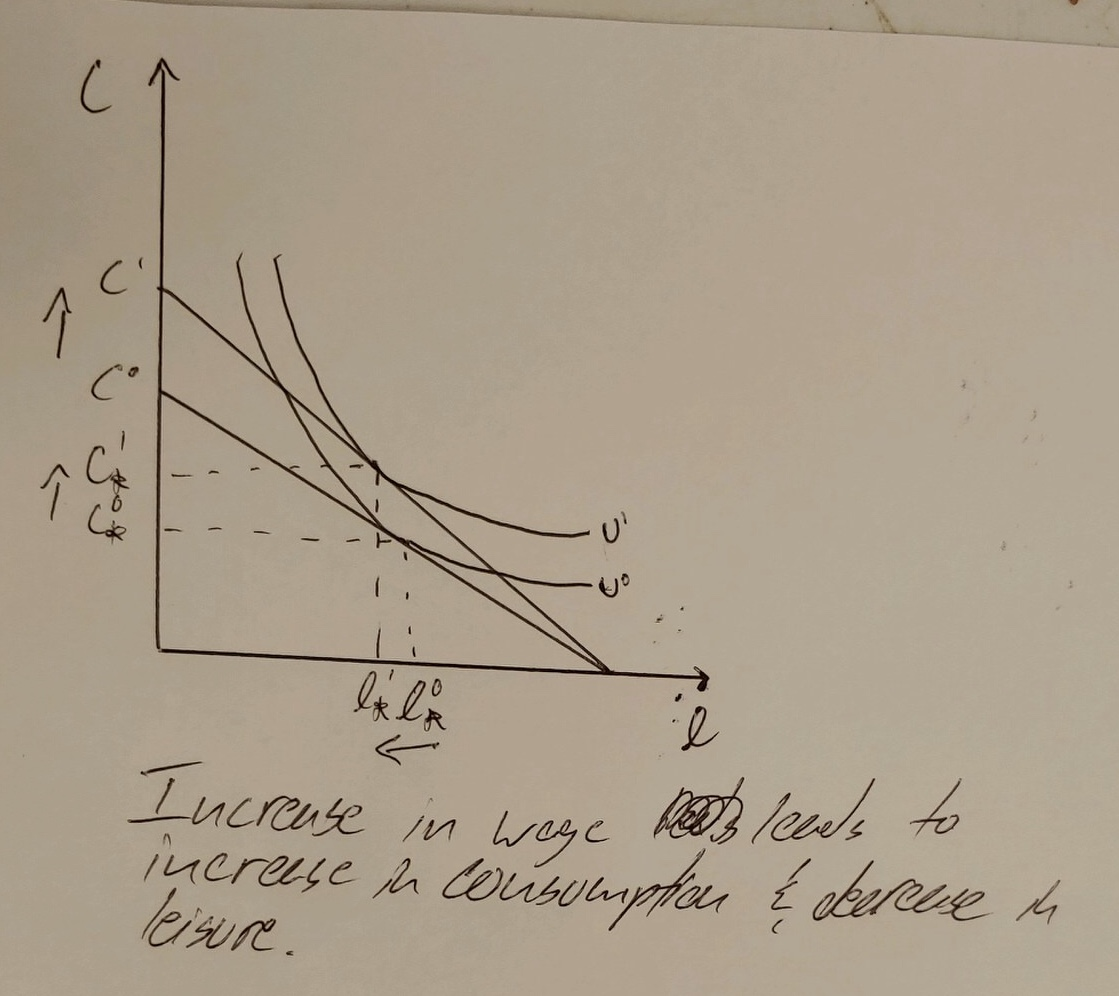
\includegraphics{2b.png}
        \end{figure}
\end{itemize}
\end{exercise}

\begin{exercise}
	\textbf{A backward-bending aggregate supply curve?} Despite our use of the backwards-bending labor supply curve as arising from the representative aganet's preferences, there is controversy in macroeconomics about whether this is a good representation. Specifically, even though a backward-bending labor supply curve may be a good description if a given individual's decisions, it does not immediately follow that the representative agent's preferences should also feature a backward-bending labor supply curve. In this exercise you will uncover for yourself one part of this proble,. For simplicity, assume that the labor tax rate is $t = 0$ throughout all that follows.
	\begin{itemize}
		\item Suppose that the economy is made up of five individuals, person A, person B, person C, person D, and person E, each of whom has the labor supply schedule given below. Using the indicated wage rates, graph each individual's labor supply curve as well as the aggregate labor supply curve.
		\begin{figure}
			\includegraphics{A-1.png}
		\end{figure}
		\begin{figure}
			\includegraphics{B-1.png}
		\end{figure}
                \begin{figure}
			\includegraphics{C-1.png}
		\end{figure}
                \begin{figure}
			\includegraphics{D-1.png}
		\end{figure}
                \begin{figure}
			\includegraphics{E-1.png}
		\end{figure}
                \begin{figure}
			\includegraphics{Agg-1.png}
		\end{figure}
\noindent Now suppose that in this economy, the "usual" range of the nominal wage is between \$10 and \$45.
		\item Restricting attention to this range, is the aggreagate labor supply curve backward-bending?
		\begin{solution}
			No,
		\end{solution}
		\begin{figure}
			\includegraphics{restAgg-1.png}
		\end{figure}
		\item At a theoretical level, if we want to use the representative-agent paradigm and restrict attention to this usual range of the wage, does a backward-bending labor supply curve make sense?
		\begin{solution}
			The backwards bend disappears when the range of wages is restriceted and aggregated. But the backwards bend still occurs for four of the five individuals within the restricted range. Hence, a model of a representative agent's behavior should include the backwards bend. 
		\end{solution}
	\end{itemize}
	Explain qualitatively the relationship you find between the individuals' labor supply curves and the aggregate labor supply curve over the range \$10 - \$45. Especially address the "backward-bending" nature of the curves.
\end{exercise}
\begin{exercise}
	\textbf{The consumption-leisure framework.} In this question you will use the basic (one-period) consumptoin-leisure framework to consider some labor market issues. Suppose that the representative consumer has the follwing utility function over consumption and labor.\\
	\indent $u(c,l) = \text{ln}c - \frac{A}{1 + \phi}n^{1+\phi}$\\
	where, as usual, $c$ denotes consumption and $n$ denotes the number of hours of labor the consumer chooses to work. The constants $A$ and $\phi$ are outside the control of the individual, but each is strictly positive. (As usual, ln($\cdot$) is the natural log function.)\\
	Suppose that the budget constraint (expressed in real, rather than in nominal, terms) the individual faces is $c = (1 - t)\cdot w \cdot n$, where $t$ is tha labor tax rate, $w$ is the real hourly wagge rate, and $n$ is the number of hours the individual works.\\
	Recall that $n + l = 1$ must always be true. The Lagrangian for this problem is\\
	\indent $\text{ln}c-\frac{A}{1 + \phi}n^{1 + \phi} + \lambda[(1 - t)wn - c]$, where $\lambda$ denotes the Lagrange multiplier on the budget constraint.
	\begin{itemize} 
		\item Based on the given Lagrangian, compute the representative consumer's first-order conditions with respect to consumption and with respect to labor. Clearly present the important steps and logic of your analysis.
		\begin{solution}
			\begin{center}
				$\mathcal{L} = \text{ln}(c) - \frac{A}{1 + \phi}n^{1 + \phi} + \lambda[(1 - t)wn - c]$\\
				$\frac{\delta \mathcal{L}}{\delta c} = \frac{1}{c} - \lambda = 0$\\
				$\frac{\delta \mathcal{L}}{\delta n} = An^\phi + \lambda(1 - t)w = 0 $\\
				$\implies \frac{1}{c} = \lambda$\\
				$\implies An^\phi = \lambda(1 - t)w$\\
			\end{center}
		\end{solution}
		\item Based on only the first-order condition with respect to labor computed in part a, qualitatively sketch two things in a diagram with the real wage on the vertical axis and labor on the horizontal axis. First, the general shape of the relationship between $w$ and $n$ (perfectly vertical, perfectly horizontal, upward sloping, downward sloping, or impossible to tell). Second, how changes in $t$ affect the relationship (shift it outward, shift it inward, or impossible to determine). Briefly describe the economics of how you obtained your conclusions. (Note: In this question you are not to use the first-order condition with respect to consumption nor any other conditions.)
		\begin{figure}
			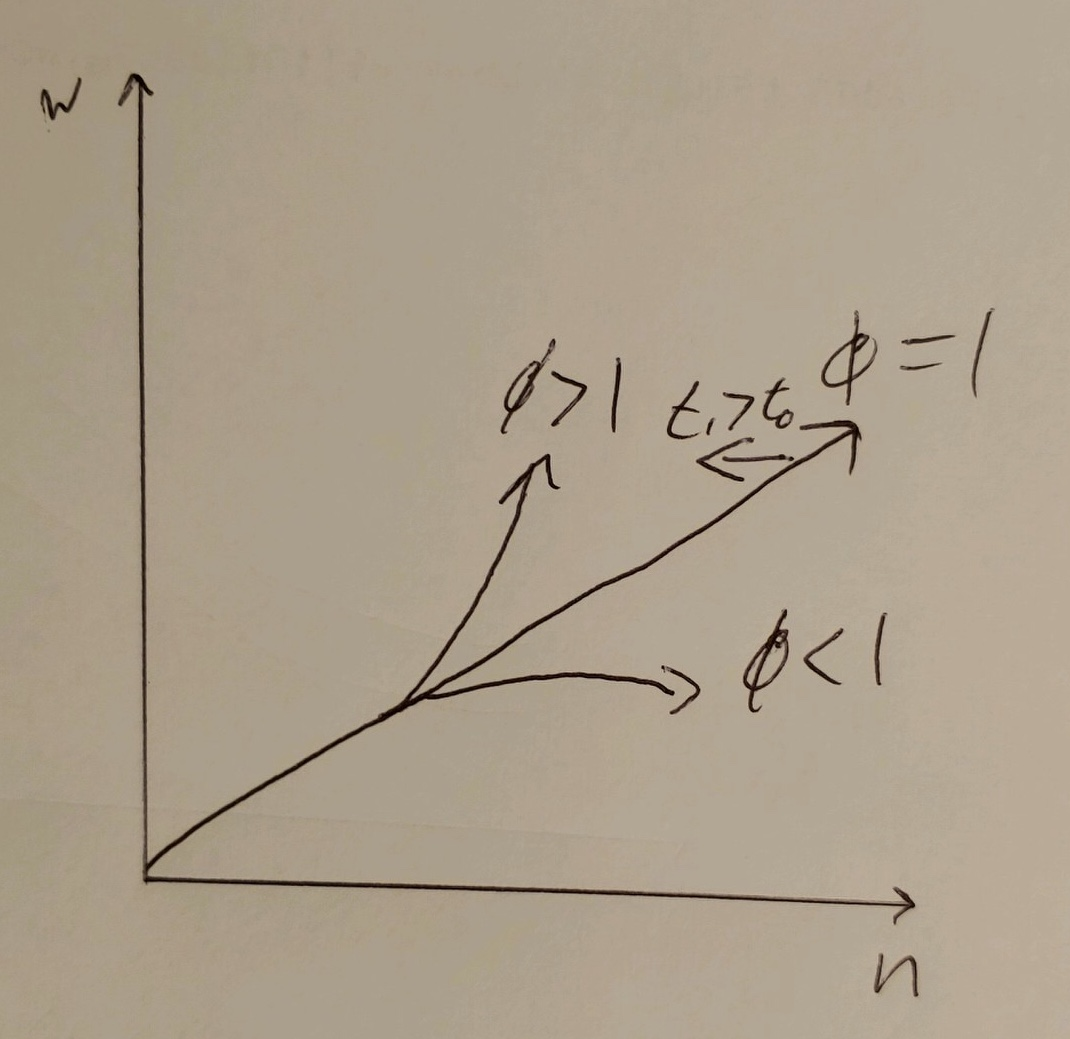
\includegraphics{4a.png}
		\end{figure}
		\begin{solution}
			\begin{center}
				$\text{FOC}_l \implies w = \frac{An^\phi}{\lambda(1 - t)}$
			\end{center}
		Based on the FOC with respect to labor we get a model similar to the one constructed below which is upward sloping. Additionally, an increase in $t$ would cause the line to shift inward. Economically, this makes sense in that, if we fix consumption, a tax increase would require more hours worked or a higher wage to remain at original consumption levels.\\
		\end{solution}
		\item Now based on both of the two first-order conditions computed in part a, construct the consumption-leisure optimality condition. Clearly present the important steps and logic of your analysis.
		\begin{solution}
			\begin{center}
				$\text{FOC's} \implies \frac{1}{cAn^\phi} = \frac{1}{(1 - t)w}$\\
				$\implies cAn^\phi = (1 - t)w$\\
				$c^* = \frac{(1 - t)w}{An^\phi}$
			\end{center}
		Substituting into the budget constraint we get
			\begin{center}
				$(1 - t)wn = c$\\
				$\implies(1 - t)wn = \frac{(1 - t)w}{An^\phi}$\\
				$\implies n = \frac{1}{An^\phi}$\\
				$\implies n^{\phi + 1} = \frac{1}{A}$\\
				$\implies n =  A^{-\frac{1}{\phi + 1}}$\\
				$\implies w = \frac{A^{\frac{1}{1 + \phi}}}{(1 + t)}$
			\end{center}
		\end{solution}
		\item Based on both the consumption-leisure optimality condition obtained in part c and on the budget constraint, qualitatively sketch two things in a diagram with the real wage on the vertical axis and labor on the horizontal axis. First, the general shape of the relationship between $w$ and $n$ (perfectly vertical, perfectly horizontal, upward sloping, downward sloping, or impossible to tell). Second, how changes in $t$ affect the relationship (shift it outward, shift it inward, or impossible to determine). Briefly describe the ceonomics of how you obtained your conclusions.
		\begin{solution}
			\begin{figure}
				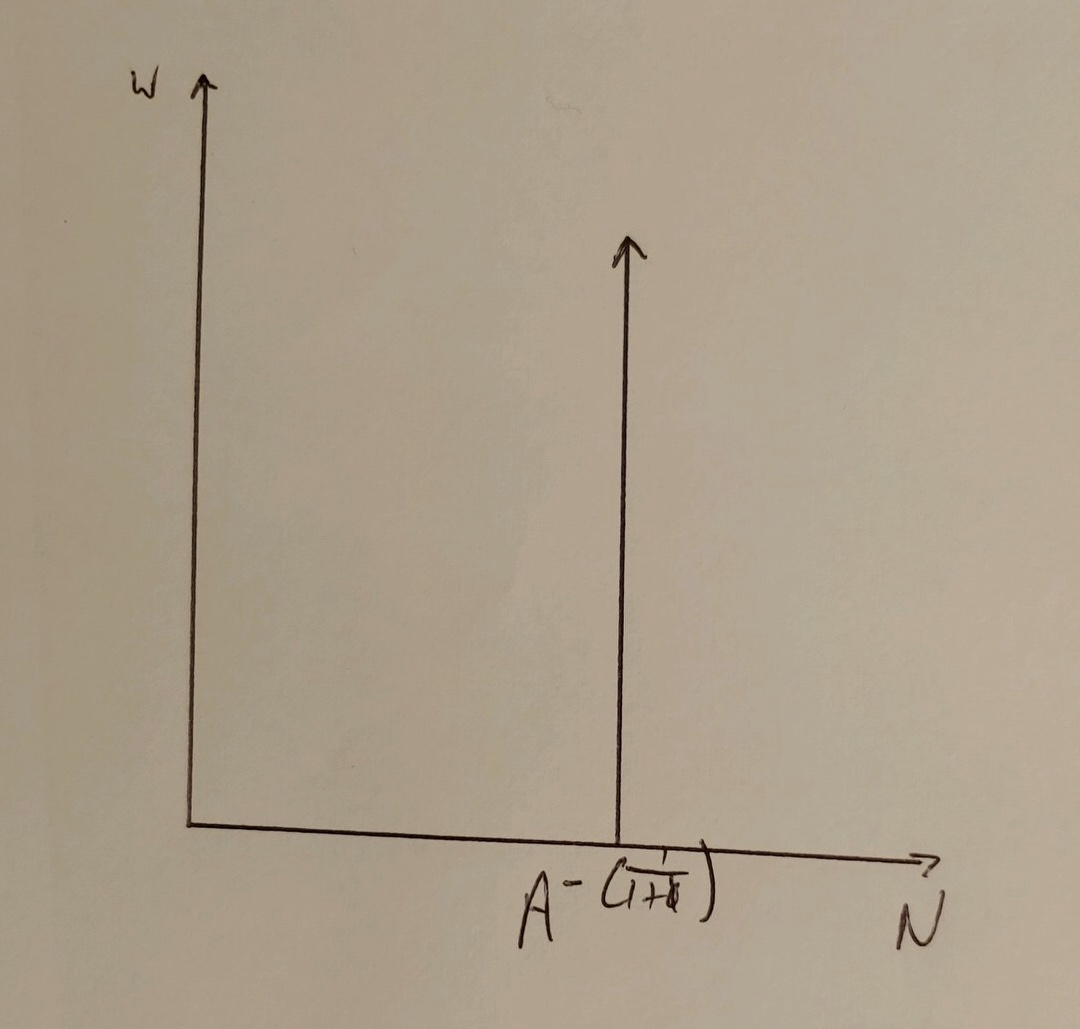
\includegraphics{4b.png}
			\end{figure}
			Because neither $w$ nor $t$ are included in the optimal hours worked function, we get a perfectly vertical line that is not affected by changes in taxes.
		\end{solution}
		\item How do the conclusions in part d compare with those in part b? Are they broadly similar? Are the very different? Is it impossible to compare them? In no more than 60 words, describe as much as you can about the economics (do not simply restate the mathematics you computed above) when comparing the pair of diagrams.
		\begin{solution}
			Due to the unconvential nature of the indifference curve, the two graphs are vastly different from each other. This is because the utility optimizing bundle is completely dependant on factors outside of the agent's control.
		\end{solution}
	\end{itemize}
\end{exercise}
\begin{exercise}
	\textbf{European and US consumption-leisure choices.} Suppose that one unit of time is 168 hours (per week). Europeans work fewer hours than Americans. There are likely very many possible reasons for this, and indeed in reality this fact arises from a conbination of many reasons. In this question you will consider two reasons using the simple (one-perid) consumption leisure model.
	\begin{itemize}
		\item Suppose that both the utility functions and before-tax real wages $W / P$ of American and European individuals are identical. However, the labor income tax rate in Europe is higher than in America. In a single carefully labeled indifference curve/budget constraint diagram (with consumption on the viertical axis and leisure on the horizontal axis), show how it can be the case that Europeans work fewer hours than Americans. Provide any explanation of your diagram that is needed.
		\begin{figure}
                        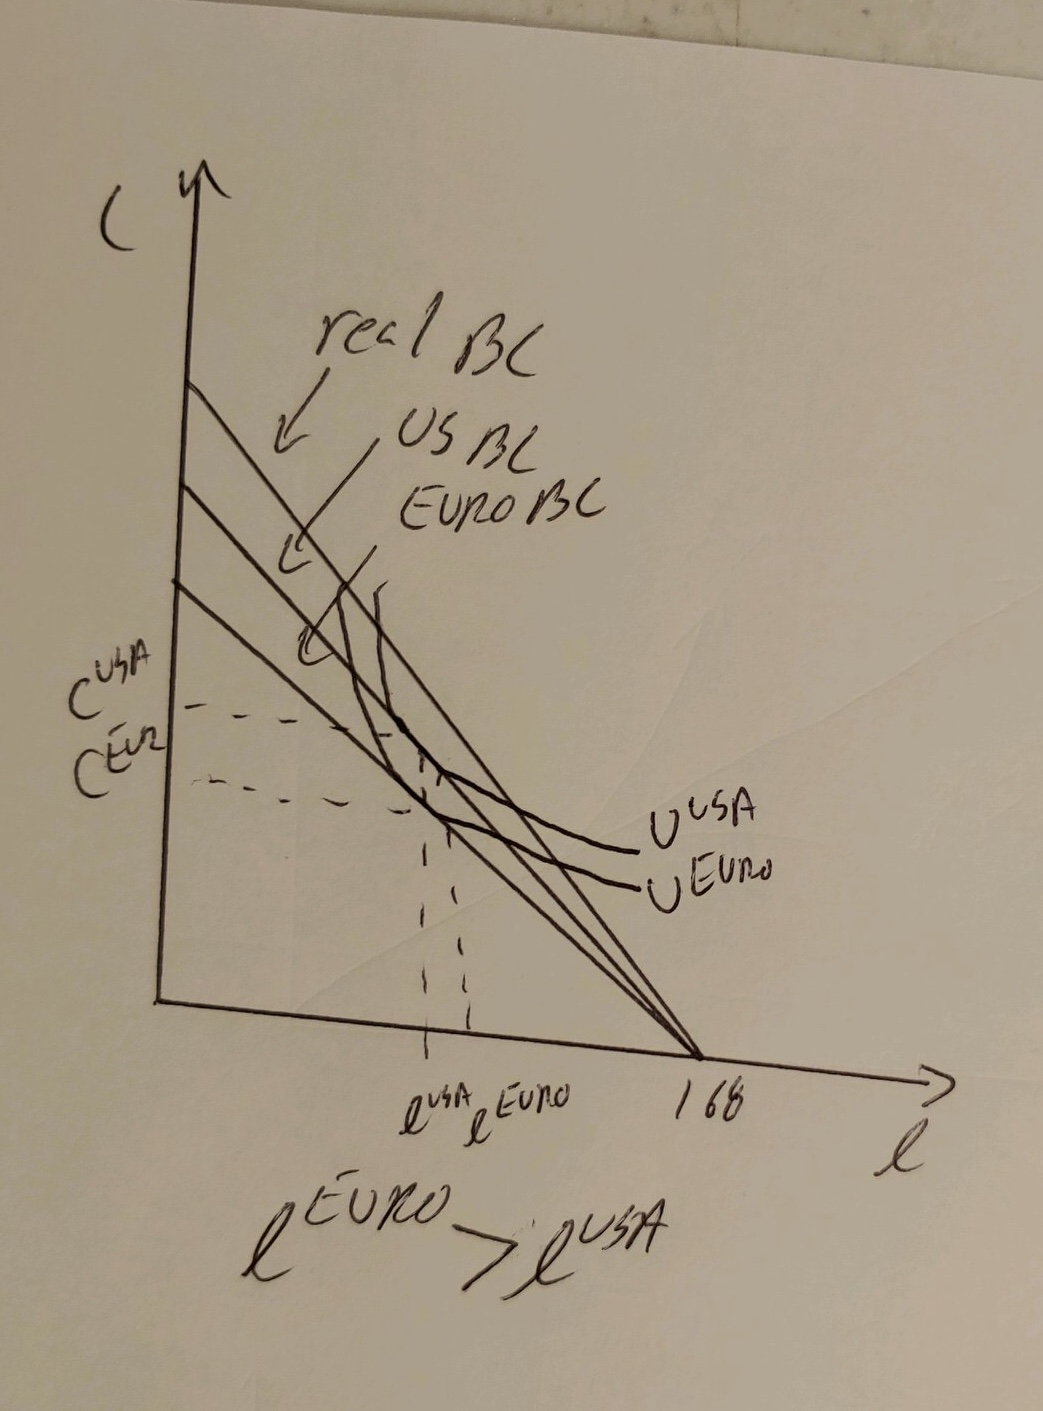
\includegraphics{5a.png}
                \end{figure}
		\item Suppose that both the before-tax real wages $w / P$ and tha labor tax rates imposed on American and European individuals are identical. However, the utility function $u^{AMER}(c,l)$ of Americans differs from that of Europeans $u^{EUR}(c,l)$. In a \textbf{single} carefully labeled indifference-curve/budget constrained diagram (with consumption on the vertical axis and leisure on the horizontal axis), show how it can be the case tha Europeans work fewer hours than Americans. Provide any explanation of your diagram that is needed. 
		\begin{figure}
			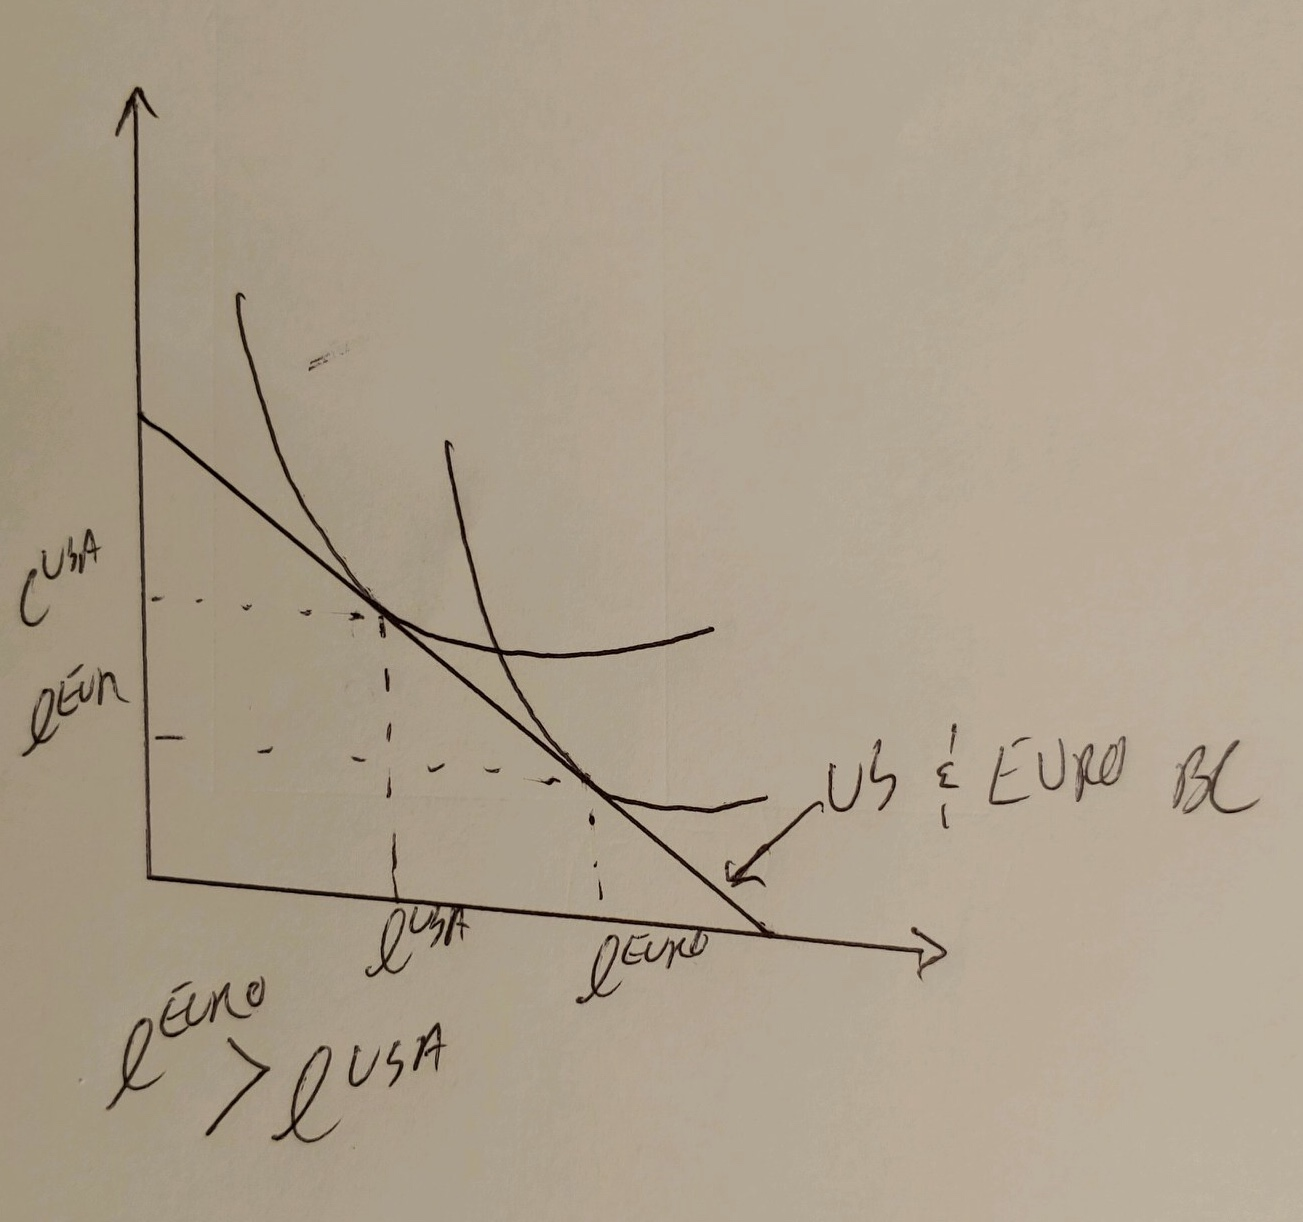
\includegraphics{5b.png}
		\end{figure}
	\end{itemize}
\end{exercise}
\begin{exercise}
	\textbf{A national service program.} Suppose that one unit of time is 168 hours (per week). Consider the following radical policy proposal: rather than taxes being levied on individuals and the proceeds of those taxes being used by the government ot fund various programs, suppose that every individuals pays no taxes of any kind but instead must give ten hours of his time every week to national service. You are to analyze this national service program in the context of the (one-period) consumption leisure framework. Thus there are now three uses of the individual's time: work, leisure, and national service (The mandatory 10 hours). Assume the following:
	\begin{enumerate}
		\item Instituting the national service program has no effect on the prices or wages in the economy.
		\item Any time spent voluntarily performing national service beyond 10 hours is considered leisure.
	\end{enumerate}
	\begin{itemize}
		\item Using the notation developed in this chapter (i.e., $c$ to denote consumption, $n$ to denote hours of work per week, $l$ to denote hours of leisure per week, $P$ to denote the nominal price of consumption, and $W$ to denote the nominal hourly wage), construct the representative agent's (weekly budget constraint in this model with the national service program. Provide brief economic justification for your work.
		\begin{solution}
			Recall the original budget constraint which had a nonzero tax rate and a time period normalized to 1.\\
			\begin{center}
				$Pc + (1 - t)wl = (1 - t)w$
			\end{center}
			Our new constrain will have a time period of $168$ hours, a tax rate of $0$, and $10$ hours of mandatory service.
			\begin{center}
				$168 - l - 10 = 158 - l$\\
				$\implies Pc = w(158 - l)$\\
				$\implies Pc + wl = w158$
			\end{center}
			The interpretation of the new budget constraint is similar to that of the original budget constraint. The left side of the equation represents the total cost of consumption and leisure while the right side represents the total income of the period. 
		\end{solution}
		\item Now recall the baseline consumption-leisure framework with no national service program. Suppose that both the consumption tax rate is zero and the labor tax rate is zero. How does the slope of the budget constraint in this economy compare with the slope of the budget constraint in the economy with the national service program in part a? Provide brief economic explanation.
		\begin{solution}
			No national service: \\
			\begin{center}
				$Pc + wl = 168w$\\
				$\implies c = \frac{w}{p}(168 - l)$
				$\implies \frac{\delta c^0}{\delta l} = -\frac{w}{p}$
			\end{center}
			National service included:
			\begin{center}
				$Pc + wl = 158w$\\
				$\implies c = \frac{w}{p}(158 - l)$\\
				$\implies \frac{\delta c^1}{\delta l} = -\frac{w}{p} = \frac{\delta c^0}{\delta l}$
			\end{center}
			So the slope remains unchanged. Economically, this is due to the fact that relative prices are held constant and the new budget constraint is created through a shift in the old one as opposed to a rotation.
		\end{solution}
	\end{itemize}
\end{exercise}
\end{document}
